\setlength{\columnsep}{3pt}
\begin{flushleft}
	\begin{itemize}
		\item A filesystem is divided into two parts – data blocks and inode number.
		\begin{figure}[h!]
			\centering
			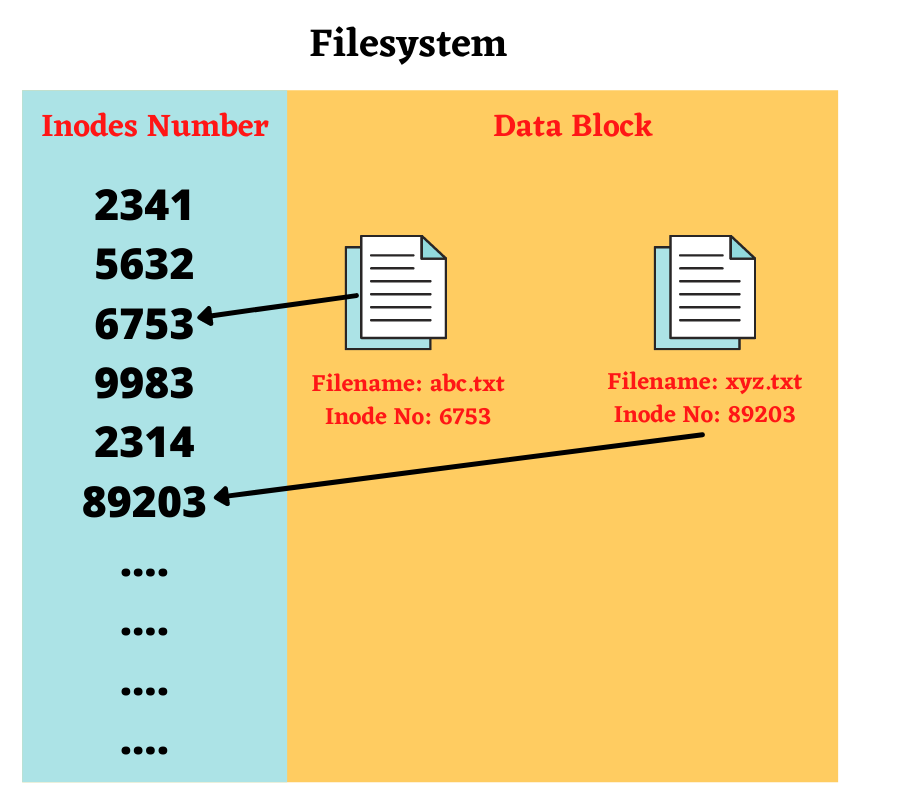
\includegraphics[scale=.5]{content/chapter10/images/inodes.png}
			\caption{Filesystem and inodes}
			\label{fig:Filesystem_inodes}
		\end{figure}
		\item How do I see a file's inode number?
		\newline
		\textbf{Solution:} You can use \textbf{"ls -i"} command to see inode number of file:
		\bigskip
		\begin{tcolorbox}[breakable,notitle,boxrule=-0pt,colback=black,colframe=black]
			\color{green}
			\fontdimen2\font=1em
			\# ls -i /etc/passwd
			\newline
			\color{white}
			32820 /etc/passwd
			\fontdimen2\font=4pt
		\end{tcolorbox}
		

	\end{itemize}	
\end{flushleft}
\newpage


